\documentclass[letterpaper,12pt]{article}
\usepackage{tabularx} % extra features for tabular environment
\usepackage{amsmath}  % improve math presentation
\usepackage{amssymb}
\usepackage{graphicx} % takes care of graphic including machinery
\usepackage[margin=1in,letterpaper]{geometry} % decreases margins
\usepackage{cite} % takes care of citations
\usepackage[final]{hyperref} % adds hyper links inside the generated pdf file
\usepackage{caption}
\usepackage{subcaption}

\hypersetup{
	colorlinks=true,       % false: boxed links; true: colored links
	linkcolor=black,        % color of internal links
	citecolor=blue,        % color of links to bibliography
	filecolor=magenta,     % color of file links
	urlcolor=blue         
}
\usepackage{blindtext}
\usepackage[utf8]{inputenc}
\usepackage[english]{babel}
\usepackage{gensymb}
\usepackage{amsthm}
\usepackage{listings}
%\usepackage{algorithm}
%\usepackage{algorithmic}
\usepackage[ruled,vlined]{algorithm2e}

\theoremstyle{plain}
\newtheorem{theorem}{Theorem}[section]
\newtheorem{lemma}[theorem]{Lemma}
\newtheorem{prop}[theorem]{Proposition}
\newtheorem*{cor}{Corollary}

\theoremstyle{definition}
\newtheorem{defn}{Definition}[section]
\newtheorem{conj}{Conjecture}[section]
\newtheorem{exmp}{Example}[section]

\theoremstyle{remark}
\newtheorem*{rem}{Remark}
\newtheorem*{note}{Note}

\usepackage{tikz}
\usetikzlibrary{fadings}
\usetikzlibrary{patterns}
\usetikzlibrary{shadows.blur}
\usetikzlibrary{shapes}
\newcommand{\Pa}{\ensuremath{\mathcal{P}}}

%++++++++++++++++++++++++++++++++++++++++


\begin{document}
	
	\title{Steiner Tree - DP Over Treewidth}
	\author{Aditya Sheth - IMT201800x \\ Rathin Bhargava - IMT2017522}
	\date{\today}
	\maketitle
	\tableofcontents
	\newpage

%    \begin{section}{Introduction}
%    
%    \end{section}
  
  %!TeX root=main.tex
\begin{section}{Introduction}
	\begin{subsection}{Intro}
	The Steiner Tree Problem in an NP-Complete Problem. It's a generalization of two polynomially solvable problem - shortest path and the minimum spanning tree. The problem is defined as follows. Given a weighted undirected graph $G$, and $T \subseteq V$, we would like to find a sub-graph of $G$ which is a tree and spans all vertices in $T$. \\
	
	It reduces to the shortest path problem on graphs if $|T|=2$ and to the minimum spanning tree if $|T|=|V|$. \\
	
	This problem is a PACE 2018 Challenge problem. 
	\end{subsection}

	\begin{subsection}{Our work}
		We implemented algorithms of both tracks involving exact algorithms - Track 1 and Track 2. Track 1 had test cases with a low number of terminals. Track 2 on the other hand had test cases with arbitrarily high number of terminals (3k) but graphs with low treewidth. \\
		
		The Track 1 algorithm was an $\mathcal{O}*(3^k)$ algorithm, where $k$ is the number of terminals. Our Track 2 algorithm is a DP over Treewidth algorithm which takes $\mathcal{O}^*(k^{O(k)})$ time. 
	\end{subsection}
\end{section}
    
   %!TeX root=main.tex
\begin{section}{Nice Tree Decomposition}
	\label{section:NTD}
	In this section, we'll go over how we converted a tree decomposition into a nice tree decomposition. 
	
	%!TeX root=main.tex

\begin{figure}
	\begin{subfigure}[b]{0.3\textwidth}
		\tikzset{every picture/.style={line width=0.75pt}} %set default line width to 0.75pt        
		\begin{center}	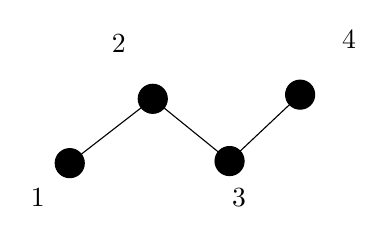
\begin{tikzpicture}[x=0.75pt,y=0.75pt,yscale=-1,xscale=1]
			%uncomment if require: \path (0,753); %set diagram left start at 0, and has height of 753
			
			%Shape: Circle [id:dp38248290994343526] 
			\draw  [fill={rgb, 255:red, 0; green, 0; blue, 0 }  ,fill opacity=1 ] (136,117) .. controls (136,113.13) and (139.13,110) .. (143,110) .. controls (146.87,110) and (150,113.13) .. (150,117) .. controls (150,120.87) and (146.87,124) .. (143,124) .. controls (139.13,124) and (136,120.87) .. (136,117) -- cycle ;
			%Shape: Circle [id:dp2739931949432536] 
			\draw  [fill={rgb, 255:red, 0; green, 0; blue, 0 }  ,fill opacity=1 ] (247,84) .. controls (247,80.13) and (250.13,77) .. (254,77) .. controls (257.87,77) and (261,80.13) .. (261,84) .. controls (261,87.87) and (257.87,91) .. (254,91) .. controls (250.13,91) and (247,87.87) .. (247,84) -- cycle ;
			%Shape: Circle [id:dp6358813933166481] 
			\draw  [fill={rgb, 255:red, 0; green, 0; blue, 0 }  ,fill opacity=1 ] (213,116) .. controls (213,112.13) and (216.13,109) .. (220,109) .. controls (223.87,109) and (227,112.13) .. (227,116) .. controls (227,119.87) and (223.87,123) .. (220,123) .. controls (216.13,123) and (213,119.87) .. (213,116) -- cycle ;
			%Shape: Circle [id:dp48939126493276053] 
			\draw  [fill={rgb, 255:red, 0; green, 0; blue, 0 }  ,fill opacity=1 ] (176,86) .. controls (176,82.13) and (179.13,79) .. (183,79) .. controls (186.87,79) and (190,82.13) .. (190,86) .. controls (190,89.87) and (186.87,93) .. (183,93) .. controls (179.13,93) and (176,89.87) .. (176,86) -- cycle ;
			%Straight Lines [id:da20589949937660657] 
			\draw    (143,117) -- (183,86) ;
			%Straight Lines [id:da9819397938135097] 
			\draw    (220,116) -- (254,84) ;
			%Straight Lines [id:da11052047537584375] 
			\draw    (183,86) -- (220,116) ;
			
			% Text Node
			\draw (123,128) node [anchor=north west][inner sep=0.75pt]   [align=left] {1};
			% Text Node
			\draw (162,54) node [anchor=north west][inner sep=0.75pt]   [align=left] {2};
			% Text Node
			\draw (220,128) node [anchor=north west][inner sep=0.75pt]   [align=left] {3};
			% Text Node
			\draw (273,52) node [anchor=north west][inner sep=0.75pt]   [align=left] {4};
			
			
			\end{tikzpicture}
		\end{center}
		\caption{$\mathcal{P}_4$}
		\label{p4}
	\end{subfigure}
	\begin{subfigure}[b]{0.3\textwidth}
		\begin{center}
			
			\tikzset{every picture/.style={line width=0.75pt}} %set default line width to 0.75pt        
			
			
			\tikzset{every picture/.style={line width=0.75pt}} %set default line width to 0.75pt        
			
			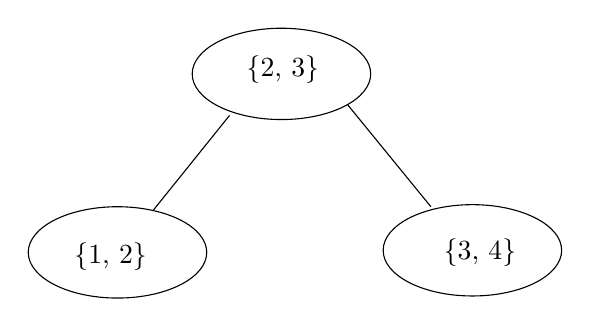
\begin{tikzpicture}[x=0.75pt,y=0.75pt,yscale=-1,xscale=1]
			%uncomment if require: \path (0,632); %set diagram left start at 0, and has height of 632
			
			%Shape: Ellipse [id:dp5175570165318644] 
			\draw   (281,83) .. controls (281,70.85) and (300.25,61) .. (324,61) .. controls (347.75,61) and (367,70.85) .. (367,83) .. controls (367,95.15) and (347.75,105) .. (324,105) .. controls (300.25,105) and (281,95.15) .. (281,83) -- cycle ;
			%Shape: Ellipse [id:dp7529479424703472] 
			\draw   (202,169) .. controls (202,156.85) and (221.25,147) .. (245,147) .. controls (268.75,147) and (288,156.85) .. (288,169) .. controls (288,181.15) and (268.75,191) .. (245,191) .. controls (221.25,191) and (202,181.15) .. (202,169) -- cycle ;
			%Shape: Ellipse [id:dp7057208736562427] 
			\draw   (373,168) .. controls (373,155.85) and (392.25,146) .. (416,146) .. controls (439.75,146) and (459,155.85) .. (459,168) .. controls (459,180.15) and (439.75,190) .. (416,190) .. controls (392.25,190) and (373,180.15) .. (373,168) -- cycle ;
			%Straight Lines [id:da698063510315667] 
			\draw    (299,103) -- (262,149) ;
			%Straight Lines [id:da6342459798451947] 
			\draw    (356,98) -- (396,147) ;
			
			
			% Text Node
			\draw (306,73) node [anchor=north west][inner sep=0.75pt]   [align=left] {\{2, 3\}};
			% Text Node
			\draw (223,163) node [anchor=north west][inner sep=0.75pt]   [align=left] {\{1, 2\}};
			% Text Node
			\draw (401,161) node [anchor=north west][inner sep=0.75pt]   [align=left] {\{3, 4\}};
			
			
			\end{tikzpicture}
		\end{center}
		\caption{Tree Decomposition}
		\label{TreeDecomp}
	\end{subfigure}
\end{figure}

\begin{figure}
	\centering
	
	
	\tikzset{every picture/.style={line width=0.75pt}} %set default line width to 0.75pt        
	
	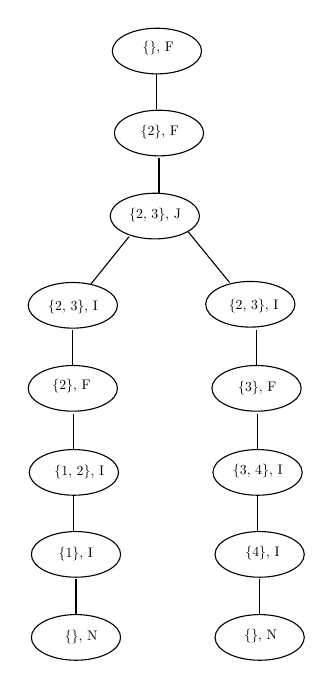
\begin{tikzpicture}[x=0.75pt,y=0.75pt,yscale=-0.5,xscale=0.5, every node/.style={scale=0.5}]
	%uncomment if require: \path (0,770); %set diagram left start at 0, and has height of 770
	
	%Shape: Ellipse [id:dp5248588589594857] 
	\draw   (250,225) .. controls (250,212.85) and (269.25,203) .. (293,203) .. controls (316.75,203) and (336,212.85) .. (336,225) .. controls (336,237.15) and (316.75,247) .. (293,247) .. controls (269.25,247) and (250,237.15) .. (250,225) -- cycle ;
	%Shape: Ellipse [id:dp8855808935720543] 
	\draw   (171,311) .. controls (171,298.85) and (190.25,289) .. (214,289) .. controls (237.75,289) and (257,298.85) .. (257,311) .. controls (257,323.15) and (237.75,333) .. (214,333) .. controls (190.25,333) and (171,323.15) .. (171,311) -- cycle ;
	%Shape: Ellipse [id:dp606634779506167] 
	\draw   (342,310) .. controls (342,297.85) and (361.25,288) .. (385,288) .. controls (408.75,288) and (428,297.85) .. (428,310) .. controls (428,322.15) and (408.75,332) .. (385,332) .. controls (361.25,332) and (342,322.15) .. (342,310) -- cycle ;
	%Straight Lines [id:da06110450839607107] 
	\draw    (268,245) -- (231,291) ;
	%Straight Lines [id:da47523090776105303] 
	\draw    (325,240) -- (365,289) ;
	%Shape: Ellipse [id:dp20858809529480138] 
	\draw   (348,391) .. controls (348,378.85) and (367.25,369) .. (391,369) .. controls (414.75,369) and (434,378.85) .. (434,391) .. controls (434,403.15) and (414.75,413) .. (391,413) .. controls (367.25,413) and (348,403.15) .. (348,391) -- cycle ;
	%Straight Lines [id:da02966169889332848] 
	\draw    (391,369) -- (391,335) ;
	%Shape: Ellipse [id:dp24948535115685688] 
	\draw   (349,472) .. controls (349,459.85) and (368.25,450) .. (392,450) .. controls (415.75,450) and (435,459.85) .. (435,472) .. controls (435,484.15) and (415.75,494) .. (392,494) .. controls (368.25,494) and (349,484.15) .. (349,472) -- cycle ;
	%Straight Lines [id:da8483719242560979] 
	\draw    (392,450) -- (392,416) ;
	%Shape: Ellipse [id:dp3104496219770304] 
	\draw   (351,551) .. controls (351,538.85) and (370.25,529) .. (394,529) .. controls (417.75,529) and (437,538.85) .. (437,551) .. controls (437,563.15) and (417.75,573) .. (394,573) .. controls (370.25,573) and (351,563.15) .. (351,551) -- cycle ;
	%Straight Lines [id:da6840204738433688] 
	\draw    (392,528) -- (392,494) ;
	%Shape: Ellipse [id:dp16734206164466903] 
	\draw   (351,631) .. controls (351,618.85) and (370.25,609) .. (394,609) .. controls (417.75,609) and (437,618.85) .. (437,631) .. controls (437,643.15) and (417.75,653) .. (394,653) .. controls (370.25,653) and (351,643.15) .. (351,631) -- cycle ;
	%Straight Lines [id:da7490825803812134] 
	\draw    (394,609) -- (394,575) ;
	%Shape: Ellipse [id:dp625252921606493] 
	\draw   (171,391) .. controls (171,378.85) and (190.25,369) .. (214,369) .. controls (237.75,369) and (257,378.85) .. (257,391) .. controls (257,403.15) and (237.75,413) .. (214,413) .. controls (190.25,413) and (171,403.15) .. (171,391) -- cycle ;
	%Straight Lines [id:da8747789462467919] 
	\draw    (214,369) -- (214,335) ;
	%Shape: Ellipse [id:dp7167438998112289] 
	\draw   (172,472) .. controls (172,459.85) and (191.25,450) .. (215,450) .. controls (238.75,450) and (258,459.85) .. (258,472) .. controls (258,484.15) and (238.75,494) .. (215,494) .. controls (191.25,494) and (172,484.15) .. (172,472) -- cycle ;
	%Straight Lines [id:da6775872899017072] 
	\draw    (215,450) -- (215,416) ;
	%Shape: Ellipse [id:dp4830312977183936] 
	\draw   (174,551) .. controls (174,538.85) and (193.25,529) .. (217,529) .. controls (240.75,529) and (260,538.85) .. (260,551) .. controls (260,563.15) and (240.75,573) .. (217,573) .. controls (193.25,573) and (174,563.15) .. (174,551) -- cycle ;
	%Straight Lines [id:da9065403939161113] 
	\draw    (215,528) -- (215,494) ;
	%Shape: Ellipse [id:dp7622433258791789] 
	\draw   (174,631) .. controls (174,618.85) and (193.25,609) .. (217,609) .. controls (240.75,609) and (260,618.85) .. (260,631) .. controls (260,643.15) and (240.75,653) .. (217,653) .. controls (193.25,653) and (174,643.15) .. (174,631) -- cycle ;
	%Straight Lines [id:da5159274806843283] 
	\draw    (217,609) -- (217,575) ;
	%Shape: Ellipse [id:dp36642109285923596] 
	\draw   (252,66) .. controls (252,53.85) and (271.25,44) .. (295,44) .. controls (318.75,44) and (338,53.85) .. (338,66) .. controls (338,78.15) and (318.75,88) .. (295,88) .. controls (271.25,88) and (252,78.15) .. (252,66) -- cycle ;
	%Shape: Ellipse [id:dp579170044821565] 
	\draw   (254,145) .. controls (254,132.85) and (273.25,123) .. (297,123) .. controls (320.75,123) and (340,132.85) .. (340,145) .. controls (340,157.15) and (320.75,167) .. (297,167) .. controls (273.25,167) and (254,157.15) .. (254,145) -- cycle ;
	%Straight Lines [id:da11334735837963827] 
	\draw    (295,122) -- (295,88) ;
	%Straight Lines [id:da07305489134692822] 
	\draw    (297,203) -- (297,169) ;
	
	
	% Text Node
	\draw (278,136) node [anchor=north west][inner sep=0.75pt]   [align=left] {\{2\}, F};
	% Text Node
	\draw (280,55) node [anchor=north west][inner sep=0.75pt]   [align=left] {\{\}, F};
	% Text Node
	\draw (267,216) node [anchor=north west][inner sep=0.75pt]   [align=left] {\{2, 3\}, J};
	% Text Node
	\draw (189,305) node [anchor=north west][inner sep=0.75pt]   [align=left] {\{2, 3\}, I};
	% Text Node
	\draw (363,304) node [anchor=north west][inner sep=0.75pt]   [align=left] {\{2, 3\}, I};
	% Text Node
	\draw (195,464) node [anchor=north west][inner sep=0.75pt]   [align=left] {\{1, 2\}, I};
	% Text Node
	\draw (199,543) node [anchor=north west][inner sep=0.75pt]   [align=left] {\{1\}, I};
	% Text Node
	\draw (205,623) node [anchor=north west][inner sep=0.75pt]   [align=left] {\{\}, N};
	% Text Node
	\draw (378,622) node [anchor=north west][inner sep=0.75pt]   [align=left] {\{\}, N};
	% Text Node
	\draw (379,542) node [anchor=north west][inner sep=0.75pt]   [align=left] {\{4\}, I};
	% Text Node
	\draw (367,463) node [anchor=north west][inner sep=0.75pt]   [align=left] {\{3, 4\}, I};
	% Text Node
	\draw (193,381) node [anchor=north west][inner sep=0.75pt]   [align=left] {\{2\}, F};
	% Text Node
	\draw (372,383) node [anchor=north west][inner sep=0.75pt]   [align=left] {\{3\}, F};
	
	
	\end{tikzpicture}
	\caption{Nice Tree Decomposition of tree in Fig. \ref{TreeDecomp}}
	\label{NiceTreeDecomposition}
\end{figure}
	
	The idea that we keep the nodes which are in the tree decomposition as is, and insert new nodes in between the older nodes in order to ``smoothen" the change from one node to another. 
	
	\begin{subsection}{Join Nodes}
			If a node has multiple children ($c$), we have to create join nodes. An easy way to do so is to duplicate the current node, add those two duplicates as children to the current node and then assign the first child to the left duplicated node. Now, we have $c-1$ children left, and we recurse on the right duplicated child. The current node is a join node. \\
			
			This procedure increases the height of the tree by $c$ if the original node had $c$ children. This is because we keep adding vertices only to the right. However, it doesn't matter as the algorithm does not depend on the depth. However if we did, we could minimise the height by making the binary tree of joined nodes balanced. \\
			
			We can refer to the example in Fig. \ref{TreeDecomp} where the node $\{2, 3\}$ has been duplicated as shown in Fig. \ref{NiceTreeDecomposition}. To make the tree nice w.r.t the duplicated node and its child, we'll go to the next subsection .
	\end{subsection}

	\begin{subsection}{Introduce and Forget Nodes}
		At this point, any node which has child with a different bag of vertices has only one child. By making the transition for that nice, we end up making the entire tree nice. \\
		
		Given nodes $X$ and $Y$, where $Y$ is the only child of $X$, we want to insert nodes between $X$ and $Y$ such that there is a nice path from $Y$ to $X$ as we go up the tree. \\
		
		To compute this, while going from $Y \rightarrow X$, we should add forget nodes for all vertices in $Y \backslash X$ and then add introduce nodes for all vertices in $X \backslash Y$. Note that this order is important. If we reverse the order, we can potentially increase the treewidth. \\ 
		
		This has been done in Fig. \ref{NiceTreeDecomposition} where we go from $\{3, 4\} \rightarrow \{2, 3\}$ in this manner. 
	\end{subsection}

	\begin{subsection}{Introduce Edge Nodes}
		After applying the above steps, we get a nice tree decomposition which adds and forgets vertices one by one. If we would like to add edges one by one as well, 
		Given an edge containing two vertices $u$ and $v$, let $f(u)$ and $f(v)$ denote the nodes where $u$ and $v$ are forgotten. Let $T_u$ and $T_v$ denote the subtrees of the tree decomposition rooted at $f(u)$ and $f(v)$ respectively. Now, it's easy to see that either $T_u \subset T_v$ or $T_v \subset T_u$ where $\subset$ denotes the ``subtree" property. If it isn't, then there is no node in common between $T_u$ and $T_v$ and that contradicts the property that there exists a bag containing $u$ and $v$ if there is an edge $(u, v)$ in the graph. 
		
		In such a scenario, without loss of generality, assume $T_v \subset T_u$. Then, we add an Introduce Edge node just before $v$ is forgotten, i.e. as a child of $f(v)$. This ensures that the graph isn't joined and the edge is only introduced once.  
	\end{subsection}
\end{section}



    
    %!TeX root=main.tex

\begin{section}{Algorithm Overview}
	In this section, we describe the DP over Treewidth algorithm in detail along with any implementation details or edge cases we had to explicitly take care of. 
	
	As defined by the nice tree decomposition, we have $4$ types of nodes as described above in Section \ref{section:NTD}. For each node, we've described the recurrence below. \\
	
	We add a terminal $u^*$ to all bags, which leads to an increase of the bag size by 1. This is done so that any solution for node $t$ we construct always has the invariant that it is covering the terminals for the sub graph corresponding to the subtree rooted at $X_t$. Otherwise, till the time we introduce our first terminal, we would've seen a portion of the graph already. Inserting a terminal node would mean that we check all possible forests to see if they can be extended to this terminal node. This is a very high number of possibilities (even though it's asymptotically the same). By adding that one node in the beginning, we prune off all these possibilities. \\
	
	We have implemented this algorithm in a top down fashion so that we only go to the required states and don't enumerate each and every possible state. Top down approaches prune the search tree and tend to be more efficient. At each step we memoise the solution. \\
	
	\begin{subsection}{Leaf Node}
		Since every bag has size one, there are two options for $X$. Either $X=\{u^*\}$ or $X= \emptyset$. Hence, we have two possible reachable DP states. $dp[t, \{u^*\}, \{\{u^*\}\}] = 0$ and $dp[t, \emptyset, \emptyset] = INF$. We can't build a solution from the second case since we don't uphold the invariant that the forest spans all the terminals introduced in the subtree of the node. 
	\end{subsection}

	\begin{subsection}{Introduce Vertex Node}
		While introducing a vertex $v$ without it's edges, we have two possibilities. If $v \in X$, then the partition should have a new block containing a single vertex $v$. This adds a new component to the forest. In this case, we recurse to the state where $v$ is not contained in $X$ and the block $\{v\}$ is not contained in $\Pa$ and recurse on that state. Otherwise, we ignore the vertex and recurse. Note that if $v$ is a terminal then $v$ has to be in $X$, otherwise it's impossible and we return $INF$. Also, if $v = u^*$, we just simply recurse to the child with the same $X$ and $\Pa$. This is because $u^*$ had already been introduced initially in every leaf node. We shouldn't introduce it again. 
		
		$$dp[t, X, \Pa] = 
		\begin{cases}
			dp[t', X \backslash \{v\}, \Pa \backslash \{\{v\}\}] & v \in X \\
			dp[t', X, \Pa] & \text{else}
		\end{cases}$$
		
	\end{subsection}

	\begin{subsection}{Forget Vertex Node}
		When we forget vertex $v$, we forget all it's edges as well. We have two possibilities here. If $v$ is not in the child solution, then we don't need to do anything. We just recurse to the child with the same $X$ and $\Pa$. We do the same if $v = u^*$ as $u^*$ can only be forgotten at the root. 
		
		If $v$ is in some child solution, then we have a variety of child states to get our answer from. Formally we check all states which include $v$ in their solution i.e. $X \cup \{v\}$. However, there can be a lot of partitions. We can generate all the child partitions by simply adding $v$ to a block in $\Pa$. Essentially, if we had $b$ blocks in $\Pa$ we are generating $b$ new partitions $\Pa'$ and recursing on them. Note that we cannot create a new block for $v$ as by doing so, we wouldn't ensure that the tree is a single connected component. 
		
		$$dp[t, X, \Pa] = 
		\min \{
			\min\limits_{\Pa'} dp[t', X, \Pa], dp[t', X \cup \{v\}, \Pa'] \}$$
	\end{subsection}


	\begin{subsection}{Introduce Edge Node}
		We add an edge $(u, v)$ in this node. If $u \notin X$ or $v \notin X$, then there's no point in adding the edge $(u, v)$ to our solution. Also, if this is not the case, but $u$ and $v$ are in different blocks in $\Pa$, then we don't add this edge either and just recurse to the child with $X$ and $\Pa$. 
		
		However, if there is a block i $\Pa$ such that $u$ and $v$ are a part of it, then we need to find suitable partitions to recurse on for the child node. Note that $X$ stays the same for the child. Let the block be $b$. Now, we need to generate partitions such that after adding the edge $(u, v)$, we get $\Pa$. All blocks except $b$ are unaffected. We can split $b$ by making two blocks, one with $u$ and the other with $v$. Now each of the other $|b|-2$ other vertices have two choices. Hence, we can generate $2^{|b|-2}$ new partitions $\Pa'$. 
		
		$$dp[t, X, \Pa] = \min\{\min\limits_{\Pa'}dp[t', X, \Pa'] + w(u, v), dp[t', X, \Pa]\} $$
	\end{subsection}

	\begin{subsection}{Join Node}
		In join nodes, $X_t = X_{t_1} = X_{t_2}$. The only change is in the partition $\Pa$. Now, we want to combine all partitions $\Pa_1$ and $\Pa_2$ such that while merging the forests from their respective solutions, we get a forest in the current solution. The only way this can happen is if no cycles are formed in this process. While we can add cycles and show that the minimum will always be a forest, by ensuring the pairs we compute the DP for merge to form a forest, we are pruning out all the cyclic merges which further optimises the solution. 
		
		The merge of two partitions $\Pa_1$ and $\Pa_2$ are said to be acyclic if $\forall u, v \in X, \nexists b_1 \in \Pa_1, b_2 \in \Pa_2$ such that $u \in b_1$ and $v \in b_1$ and $u \in b_2$ and $v \in b_2$. This is because if $\exists b \in \Pa$ where $u \in b$ and $v \in b$, then it implies that they are connected indirectly via a path in $G_t$. This is because the only time we merge two blocks into one is in introduce edge node. 
		
		In this case, that would imply that there is a path from $u$ to $v$ in $G_{t_1}$ and in $G_{t_2}$ which forms a cycle when the two forests are merged into $G_t$. 
		
		The calculation of such pairs for each partition has been described below in Section \ref{section:Partition}. This generates all partitions for vertices in the range $[0 \dots n]$. For example, the pairs of the partition is $\{\{0\}, \{1, 2\}\} \rightarrow (\{\{0\}, \{1, 2\}\}, \{\{0\}, \{1\}, \{2\}\})$. Now if the set $X = \{1, 3, 4\}$, then the pairs for the partition $\{\{1\}, \{3, 4\}\} \rightarrow  (\{\{1\}, \{3, 4\}\}, \{\{1\}, \{3\}, \{4\}\})$ can just be mapped from the earlier case since the structure of the partition is the same. 
		
		$$dp[t, X, \Pa] = \min\limits_{\Pa_1, \Pa_2} \{dp[t', X, \Pa_1] + dp[t', X, \Pa_2] \}$$
	\end{subsection}

	\begin{subsection}{Weird Nodes}
		Since the tree decompositions given in the input weren't the most optimal, there were times when the bags were repeated. As in, the contents of two bags in the tree decomposition were the same and they were connected by edges. Ideally, we would like to merge them, but that would've greatly altered the nice tree decomposition algorithm explained in Section \ref*{section:NTD}. This is because such a node couldn't be classified into the 4 regular nodes since there's no chance in the bag. Hence, we decided to keep them as is, make join nodes if necessary and just simply call the recurrence for the child. 
		
		$$dp[t, X, \Pa] = dp[t', X, \Pa]$$
	\end{subsection}

	\begin{subsection}{Running Time Analysis}
		If the treewidth is $k$, then the bag size is $k+2$ (We added one terminal node to each bag). The total work done in each (non-join) node is $O(k^k * 2 ^ k * nlogn)$. In each join node however, $k^{2k}$ because we are recursing over all pairs whose acyclic merge forms the node. The total time complexity is $O(k^{O(k)})$. However, in practice it's a little better since $k=6$ worked under 5 minutes. If we do calculate $8^16$ (taking $k+2$), that's over 1e14 instructions which would take over a day to compute. 
		
		The $k^k$ for the join node is actually $B(n)$ which is the $n^{th}$ Bell number. Hence, the bound for each join node cannot be more than $B(k+2)^2$. Asymptotically however, the time complexity is the same. 
	\end{subsection}

\end{section}
    
    %!TeX root=main.tex
\begin{section}{Generating Partition Pairs for Join Node}
	\label{section:Partition}
	In the DP recurrence for join node, given a partition $\Pa$, we need to find all pairs of partitions $\Pa_1$ and $\Pa_2$ such that the acyclic merge of $\Pa_1$ and $\Pa_2$ form $\Pa$. 
	
	\begin{subsection}{Generating Partitions}
		We can generate partitions recursively. Let $\Pa_n$ denote the set of all partitions of $n$ numbers. Each partition is made up of \textit{blocks}. A set of mutually disjoint blocks which collectively exhausts $n$ numbers forms a partition. \\
		
		To generate $\Pa_n$, we can do so recursively by first generating $\Pa_{n-1}$. Now, for each partition $p \in \Pa_{n-1}$, for each block $b \in p$, we append $\{n\}$ to that block and call the resulting partition a new partition. Lastly, we make a block from $\{n\}$ add add that to the partition $p$. Hence, if $p$ has $c$ blocks, we would've created $c+1$ new partitions from it. \\
		
		For example, consider $\{\{0, 1\}, \{2\}\} \in \Pa_2$. Now, from this partition, we can create 3 more partitions after adding the number 3. They are - $\{\{0, 1, 3\}, \{2\}\},\ \{\{0, 1\}, \{2, 3\}\}$ and $\{\{0, 1\}, \{2\}, \{3\}\}$. \\
		
		This process takes $O(B(n))$ where $B(n)$ is the $n^{th}$ bell number. Practically, we were able to generate partitions up to 12 in less than 5 minutes. 
	\end{subsection}

	Now, we go over all pairs of the partitions formed above. For each pair, we would like to see if an acyclic merge is possible, and if it is then what partition is the result of the merge. By keeping a record of the pair of partitions and the merged partition, we can build a map when given a partition, we return the list of pairs of partitions which when merged form the given partition. \\
	
	This is really useful because instead of enumerating over all possible ways of getting pairs $p_1$ and $p_2$ for a partition $p$ in a join node, we can just look up this table and recurse to the correct states without wasting computation time to check if the partitions formed are legitimate or not. \\
	
	\begin{subsection}{Acyclic Merge}
		Given two partitions $p_1$ and $p_2$, we need to check if their merge is acyclic and then actually merge the two partitions. Recall that a block in a partition represents a connected component. Hence, if two vertices belong to the same connected component in $p_1$ and $p_2$, after the merge we will form a cycle. \\
		
		To prevent this, we could simply enumerate over all possible pairs of vertices and check if they belong to the same block in both the partitions or not. This takes $O(k^2)$ where $k-1$ is the treewidth of the graph. We could optimise this further to $O(k*\alpha(k))$ by using the DSU data structure. \\
		
		The idea is that we could think of $p_1$ as a graph where each block is a connected component and add that to the data structure. This can be done in Now, for each block in $p_2$ all the vertices have to belong to different components. If not, by merging the two partitions, we create a cycle. This check can be done in $O(b * \alpha(b))$ time overall, where $b$ is the size of the block. Summing over all blocks, we can do this in $O(k * \alpha(k))$. Hence, the overall time taken is $O(k * \alpha(k))$. \\
		
		Finally, if the above conditions are satisfied and the two partitions can be merged, we can treat $p_2$ as a graph where each block is a connected component and accordingly add the edges to the DSU. Since $p_1$ is already added, all vertices connected in the DSU form a new block. Let's see an example. \\
		
		We want to merge partitions $\{\{0, 1\}, \{2\}\}$ and $\{\{0\}, \{1, 2\}\}$. Now, note that their merge is acyclic. When we add $p_1$ to the DSU initially, 0 and 1 form one component while 2 forms its own second component. Now, when we add $p_2$, since 1 and 2 are connected in $p_2$, once we add that edge, 2 gets connected to 1 resulting in one single block $\{\{0, 1, 2\}\}$ which is the result of merging our partition. 
	\end{subsection}

	Since we are checking this merge condition for every pair of vertices, this entire procedure of generating pairs takes $O(B(k)^2 * k * \alpha(k))$. Practically, we could run it for $k \leq 8$ under 5 minutes. 
\end{section}
    
    \begin{section}{Implementation}
    
    \end{section}
    
    \begin{section}{DP with low terminals (Track 1)}
    
    \end{section}
    
    %!TeX root=main.tex
\begin{section}{Observations}
	We created 11 sample test cases of small graphs of around 2-10 nodes ranging from a weighted $C_5$ to a $P_4$.  We individually verified each case and concluded that they were correct. \\
	
	\begin{subsection}{PACE Dataset Observations}
	We then ran our program on the testcases in the PACE dataset. We were able to run 14 tests successfully within the time limit of 30 minutes. \\
	
	We were only able to run tests with $k \leq 6$. All other testcases had a higher treewidth. This is because the bag size becomes $8$, and the join node takes up a lot of computation time because we go through all $B(k)$ partitions pairwise to compute their acyclic merges. When the bag size is 9, $B(k) = 21147$, where $\binom{B(9)}{2}$ is huge to store in memory (takes around 700MB). Hence, reading and writing from this pre computed structure takes a lot of time on our PCs. \\
	
		We believe with a dedicated engine (like an online judge), our performance would be better. \\
	
		It's worth noting that the participants in the actual PACE 2018 Challenge, either implemented the $O(2^k)$ algorithm or implemented the current algorithm, but switched to a more efficient one when the treewidth crossed a certain threshold. \\
	
	\begin{figure}
		\centering
		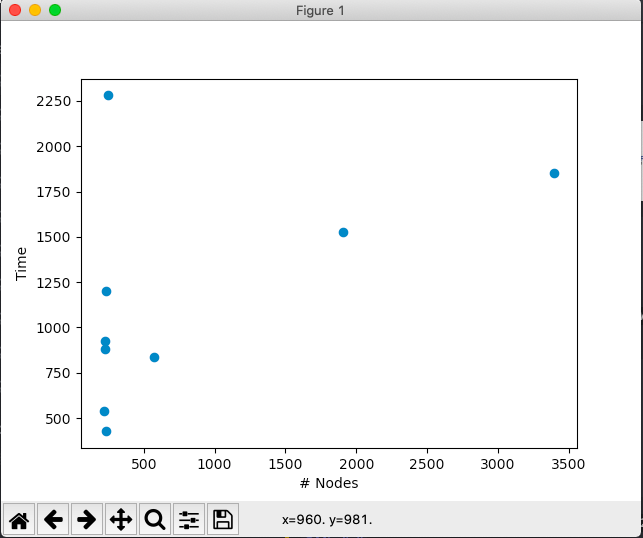
\includegraphics[scale=0.5]{NodeGraph.png}
		\caption{Plot of $|V(G)|$ vs time}
		\label{fig:nodegraph}
	\end{figure}

	While analysing the amount of time each testcase (instances 6 - 14 from PACE 2018 dataset), we realised that while the time taken to compute the optimal weight increased as the graph size increased, there was no direct relation showing so. As it can be seen in Fig. \ref{fig:nodegraph}, there are small graphs which have similar sizes (around 250 vertices) but tend to take different times. \\
	
	Since this was unusual, we ended up plotting different graphs for edges vs time and vertices * edges vs time to see if there was any difference and there wasn't. These plots looked like Fig. \ref{fig:nodegraph}. \\
	
	Our next hypothesis was that since Join Nodes tend to take more time to compute, there might be more join nodes in the graphs which take more time. This is because the treewidth is the same amongst the test cases we are considering. However, even this plot looked exactly like Fig. \ref{fig:nodegraph}. \\
	
	The reason was that while the treewidth is the same for all graphs, the join nodes in some graphs could have a smaller bag size than some other graphs. Hence, graphs with more join nodes with bigger bag sizes (but limited by treewidth) should take more time. To compute this, we summed up $|B|^|B|$ over all bags $B$ of the Join Nodes in the nice tree decomposition. We got the graph in Fig. \ref{fig:joingraph}. As we can see, there is a clear increase in time as this weighted sum increases. This also shows that the running time is asymptotically $O(k^O(k))$.  \\
	
	\begin{figure}
		\centering
		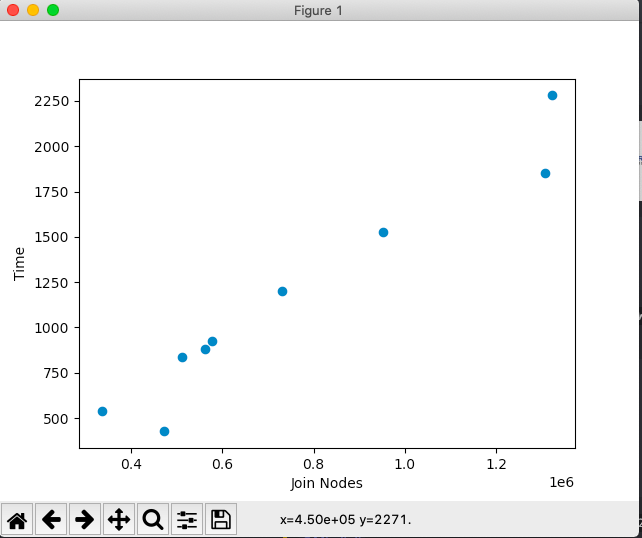
\includegraphics[scale=0.5]{JoinGraph}
		\caption{Weighted sum of Join Nodes vs time}
		\label{fig:joingraph}
	\end{figure}
	

	\end{subsection}

	This algorithm could not be tested on the track A dataset since the tree decompositions weren't given. 
	
\end{section}
    
    \begin{section}{Conclusions}
        
    \end{section}
    
	\bibliographystyle{unsrt}
	\bibliography{biblio}
	
	
\end{document}

